\usetikzlibrary{matrix}
\usetikzlibrary{positioning,arrows}
\usetikzlibrary{through}
\usetikzlibrary{calc}
\usetikzlibrary{shapes,arrows}

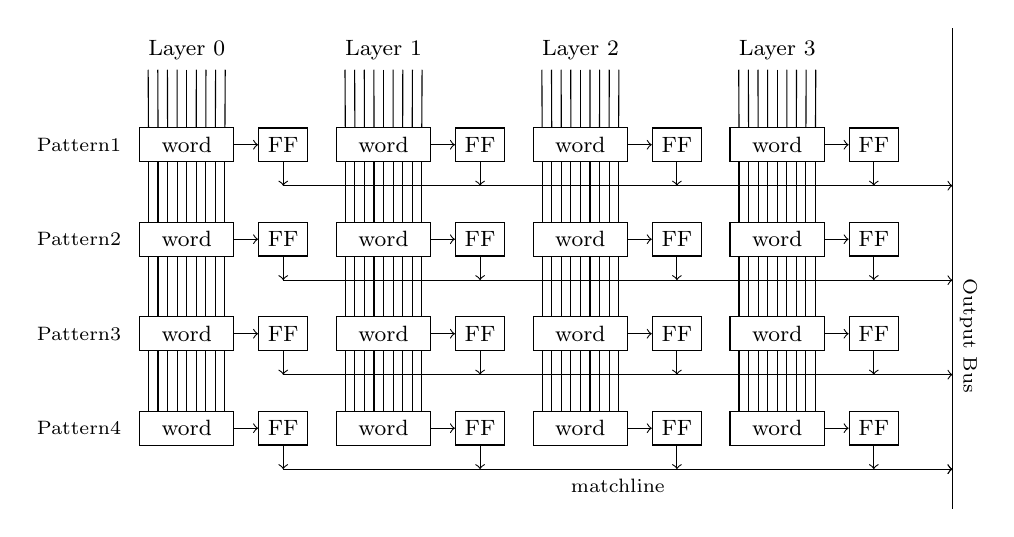
\begin{tikzpicture}

\tikzstyle{every node}=[rectangle, draw]
\tikzstyle{blank} = [coordinate]


    \foreach \x in {0,1,2,3} {
        \node[draw=none,minimum width=12mm] at (2.5*\x,0) (word\x0) {\footnotesize Layer \x};
}

 \foreach \y in {1,2,3,4} {
    \foreach \x in {0,1,2,3} {
        \node[minimum width=12mm] at (2.5*\x,-1.2*\y) (word\x\y) {\footnotesize word};
        \node[right=3mm of word\x\y] (ff\x\y){\footnotesize FF};
	\node[blank, below=3mm of ff\x\y](blank\x\y){};
	\draw[->](word\x\y) -- (ff\x\y);
	\draw[->](ff\x\y) -- (blank\x\y);
    }
\node[draw=none, left=1mm of word0\y](cell\y){\scriptsize Pattern\y};
\node[blank,right=10mm of blank3\y](blankbus\y){};
\draw[->](blank0\y) -- (blankbus\y);


}
\draw[->](blank04) -- (blankbus4) node[midway,below, draw=none]{\scriptsize matchline};

\node[blank,above=20mm of blankbus1](blankbus0){};
\node[blank,below=5mm of blankbus4](blankbus5){};
\draw[-](blankbus0) edge node [draw=none,right=2mm,rotate=-90] {\scriptsize Output Bus} (blankbus5);


 \foreach \y in {0,1,2,3} {
    \foreach \x in {0,1,2,3} {
\pgfmathtruncatemacro\next{\y+1}
\foreach \d in {0.1,0.2,0.3,0.4,0.5,0.6,0.7,0.8,0.9} {
\path (word\x\y.south west) -- (word\x\y.south east) coordinate[pos=\d] (a);
\path (word\x\next.north west) -- (word\x\next.north east) coordinate[pos=\d] (b);
\draw[] (a) -- (b);
}}
}

\end{tikzpicture}